\section{Complete times and coverage through thirteen loops}
\label{sec:notes-fast-results}
The initial fast-implementation comparison tests the direct finite products, faster exact recurrence, and newly trained recurrence strategy together with the retained sparse-seed model. The preceding deployed application is the main practical control. A matched native control retains the earlier exact formulas and block splitting but uses native Kira decisions for the remaining work. The fast fixed control uses the new exact implementation and fixed choices. Thus the native control already contains acceleration, and its timing is not the time of stock Kira on every target.

The reserved set contains 65 requests, including analytic vacuum and propagator families at every loop count through thirteen, distinct triangle products, rational scalar polygons, symbolic bubbles, and coupled native cases. Appendix~\ref{app:notes-fast-inputs} defines the targets and parameter profiles. Each method starts a fresh process three times per completed request. The timer includes loading, prediction, exact reduction, output, and the independent coefficient check. Prepared master indices and reference calculations remain separate. Table~\ref{tab:notes-fast-results} compares only requests that complete every repetition for both methods.

\begin{table}[!htbp]\centering\small
\caption{Complete application times in the new reserved test. Times are sums of per-request medians in seconds. Each row uses the same matched requests for its three controls when all methods complete; any unequal counts are reported below.}
\label{tab:notes-fast-results}
\begin{tabularx}{\linewidth}{@{}Yrrrrr@{}}\toprule
Collection & $N$ & New learned & Previous & Native & Fast fixed\\\midrule
Vacuum and propagator formulas & 26 & 5.067 & 21.963 & 21.568 & 4.912 \\
Symbolic one-mass vacua & 4 & 0.750 & 2.728 & 2.705 & 0.791 \\
Distinct triangle products & 13 & 3.604 & 4.279 & 52.016 & 3.414 \\
Scalar recurrence & 9 & 2.733 & 8.716 & 15.223 & 2.727 \\
Nonplanar seed model & 8 & 39.518 & 38.883 & 66.601 & 42.392 \\
Symbolic native inputs & 2 & 1.608 & 1.269 & 1.448 & 1.574 \\
Coupled compatibility & 3 & 3.664 & 3.737 & 3.806 & 3.696 \\
All matched requests & 65 & 56.945 & 81.574 & 163.366 & 59.505 \\
\bottomrule\end{tabularx}\end{table}

The combined method uses 30.2\% less time than the preceding deployed application, with time ratio 0.698 and repetition interval $[0.676,0.717]$. The combined method uses 65.1\% less time than the already accelerated native control, with time ratio 0.349 and repetition interval $[0.338,0.360]$.

The combined method uses 4.3\% less time than the fast fixed control, with time ratio 0.957 and repetition interval $[0.925,0.986]$. This last comparison isolates request-dependent learned choices after the exact implementation changes. It does not assign the finite-product or arithmetic savings to ML.

The combined method completes 65 of 65 requests in all three repetitions. The preceding, native, and fast fixed methods complete 65, 65, and 65 requests, respectively. Independent reference preparation takes 432.328 seconds. Across the timed runs, the exact checker performs 12,180 coefficient comparisons. The new method's first-attempt total is 59.453 seconds, including 0.000 seconds spent on unverified or incomplete first attempts. Failed requests remain in these counts and receive no completed-time speedup.

\subsection{What the new learned decision adds}
The recurrence model selects a strategy before the exact substitutions begin. Validation chooses a depth-5 tree, minimum leaf population 3, and prediction margin 0.10. Its fixed alternative selects the last raised index. The measured validation recurrence total changes from 2.6229 to 2.5000 seconds, including prediction overhead. The reserved application test admits the new model on 22 requests and changes the fixed pivot strategy on 3 requests. These groups describe observed use, while the complete scalar-recurrence group was specified before testing.

For the nine reserved scalar-recurrence requests, the combined method uses 0.2\% more time than the same fast recurrence with fixed strategy, with time ratio 1.002 and repetition interval $[0.959,1.076]$. The interval includes equal times. For the eight nonplanar requests, the combined method uses 6.8\% less time than the fixed sparse-seed choice, with time ratio 0.932 and repetition interval $[0.888,0.961]$. The latter model retains its earlier training. These comparisons separate the new recurrence decision from the retained seed decision.

\begin{figure}[!htbp]\centering
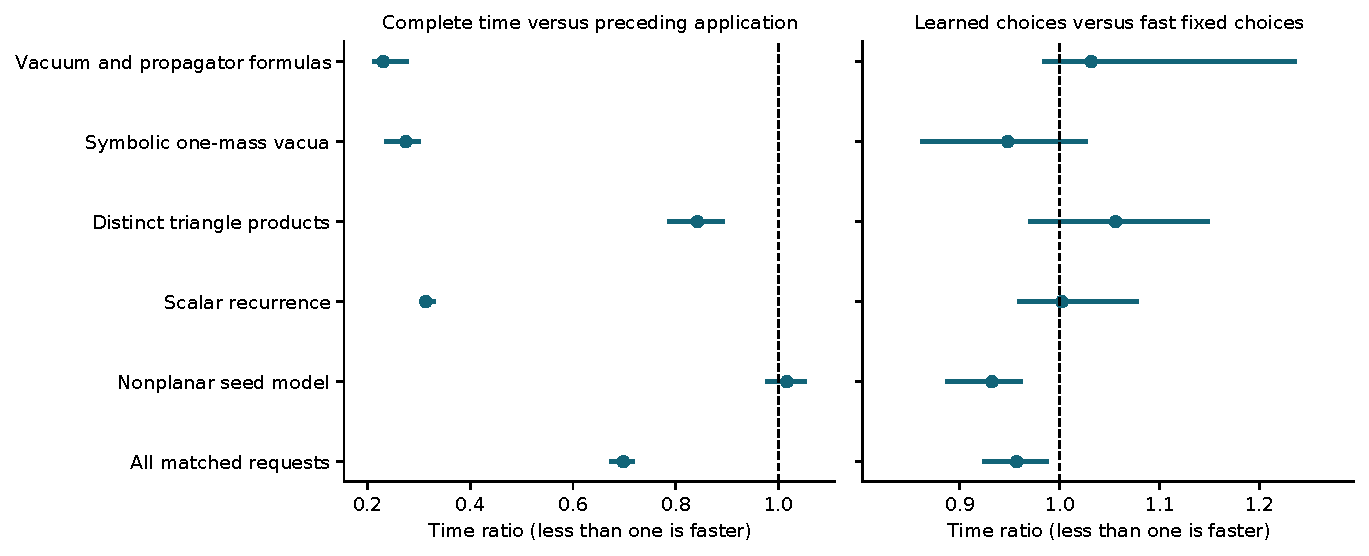
\includegraphics[width=\linewidth]{paper_figures/fast_decomposition.pdf}
\caption{Direct formulas and exact arithmetic reduce complete time, while the fixed control isolates the additional learned choices. Values below one favor the new learned application. Intervals resample the three paired repetitions on the same fixed requests. They do not measure uncertainty over all possible integral families. Formula-only groups use the same exact path in both methods, so their differences measure timing variation.}
\label{fig:notes-fast-time}
\end{figure}

\subsection{Which high-loop requests complete}
The timing set deliberately contains analytically supported families. To expose its limits, a separate 110-request audit includes one-mass and all-mass vacua, massless and massive propagators, scattering ladders, and boxes with bubble chains at each loop count through thirteen. It adds scaleless cases, other scattering structures, and symbolic scales. Each application receives twenty seconds per request. Figure~\ref{fig:notes-fast-coverage} shows the regular loop sequences, and Table~\ref{tab:notes-fast-coverage} includes every audit request.

\begin{table}[!htbp]\centering\small
\caption{Bounded audit at each loop count. ``New'' and ``Previous'' count reported completions within twenty seconds. ``Agree'' counts paired completions with exact coefficient agreement. The audit has different limits and targets from the timing comparison.}
\label{tab:notes-fast-coverage}
\begin{tabular}{@{}rrrrr@{}}\toprule
Loops & Requests & New & Previous & Agree\\\midrule
1 & 12 & 12 & 12 & 12 \\
2 & 12 & 12 & 12 & 12 \\
3 & 10 & 8 & 8 & 8 \\
4 & 7 & 4 & 4 & 4 \\
5 & 7 & 4 & 4 & 4 \\
6 & 10 & 5 & 5 & 5 \\
7 & 7 & 3 & 3 & 3 \\
8 & 7 & 3 & 2 & 2 \\
9 & 7 & 3 & 2 & 2 \\
10 & 7 & 3 & 2 & 2 \\
11 & 7 & 3 & 2 & 2 \\
12 & 7 & 3 & 2 & 2 \\
13 & 10 & 5 & 4 & 4 \\
Total & 110 & 68 & 62 & 62 \\
\bottomrule\end{tabular}\end{table}
\begin{figure}[!htbp]\centering
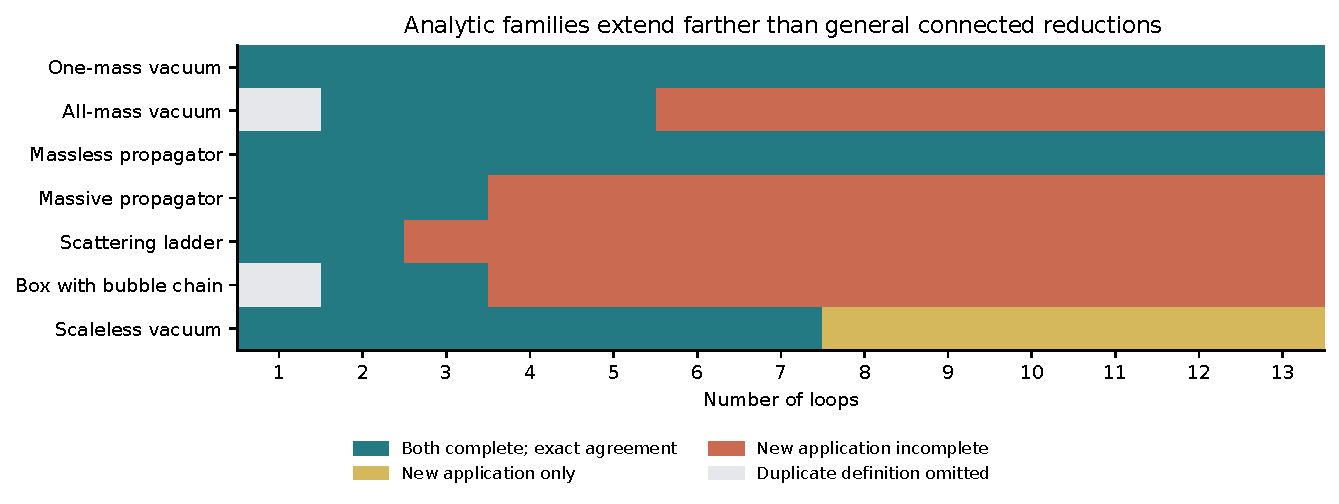
\includegraphics[width=\linewidth]{paper_figures/fast_coverage.pdf}
\caption{Completion depends on integral structure as well as loop count. The grid shows the new and preceding applications under the same twenty-second audit limit. A failed entry includes timeouts and unsupported inputs. Additional symbolic and scattering requests appear in the complete counts of Table~\ref{tab:notes-fast-coverage}.}
\label{fig:notes-fast-coverage}
\end{figure}
\FloatBarrier

The 42 incomplete requests comprise 12 time limits and 30 inputs above the native index bound.

The six additional completions are scaleless vacuum requests at eight through thirteen loops. Their exact result is zero by the homogeneous IBP identity derived in Eq.~\eqref{eq:notes-fast-scaleless}. The preceding application rejects their native index count before using this general zero rule. These additional completions come from an exact identity and carry no ML speedup claim.

The analytic families and independent products establish high-loop coverage within their derived domains. General coupled scattering, arbitrary numerator powers, singular kinematics, cut integrals, and symbolic indices require further methods or tests. The native 31-index limit also excludes some complete coupled coordinate systems~\cite{Kira3}. Neither prediction nor a shorter failed attempt supplies the missing reduction. The audit therefore records these limits explicitly and does not label its finite collection as all integral types.
